\documentclass[../ala_hataile.tex]{subfiles}
\begin{document}
	\clearpage
	\includepdf[pages=2-7, pagecommand={}]{sisasivut_19062018.pdf}
	\twocolumn[\section{Physicum}]
	Se on valmistettu betonista, lasista ja teräksestä.
	Pihalla on seinän kokoinen taideteos
	Linnunradan lähiavaruudesta. Katolla
	on hassu valkoinen pallo. Ken raskaista
	kaksinkertaisista puuovista on sisään käynyt,
	on saapunut Physicumiin.
	
	Vuodesta 2001 alkaen fysikaalisten tieteiden,
	maantieteen ja geotieteiden opiskelijoiden
	kotina toiminut Physicum ei ole oikein
	mistään kulmasta kaunis tai erityisen
	kotoisa rakennus, mutta silti siitä on vuosien
	myötä jotenkin oppinut pitämään. Ainakin
	se kertoo hyvin konkreettisella tavalla
	valtion kuluttaneen aika monta miljoonaa
	euroa saadakseen fyysikot ajettua muiden
	luonnontieteilijöiden tapaan Kumpulaan,
	pois keskustan humanisteja kiusaamasta.
	
	Physicumin yhteydessä sijaitsee myös
	Kumpulan tiedekirjasto, josta pitäisi löytyä
	suunnilleen kaikki matemaattis-luonnon\-tieteellisessä
	tiedekunnassa opiskelevan
	tarvitsemat kirjat. Kirjaston alakerrassa,
	sisäänkäynnin edessä vasemmalla on hyödyllinen
	hyllykkö, joka
	sisältää useimmat peruskursseilla käytössä olevat oppikirjat. Tiedekirjastosta
	löytyy luonnollisesti hiljaista
	työskentelytilaa, mutta myös ryhmä\-työskentely\-huoneita,
	joihin voi porukalla kokoontua
	vaikka laskareiden tekoa varten.
	Tiedekirjasto uusii kokoelmiaan vuosittain,
	joten hyväkuntoisiakin oppikirjoja annetaan
	yleensä ilmaiseksi halukkaille.
	Kannattaakin välillä käydä vilkuilemassa kirjaston poistohyllyä, sillä
	uusina alan kirjat ovat melkoisen kalliita.
	
	Sisälle Physicumiin asti uskaltautunut
	opiskelija löytää itsensä huiman korkeasta
	aulasta. Oikealla, ylös johtavien portaiden
	takana, satunnainen matkailijamme näkee
	Unicafe Physicumin, jossa ei tarjoilla
	lounasta. Mikäli nälkä yllättää ja matka
	Chemicumiin tai Exactumiin tuntuu nälkään
	nääntyvästä opiskelijarukasta liian
	pitkältä, kotoinen kahvilamme tarjoaa opiskelija-alennuksen salaateista sekä patongeista ja panineista
	(kera pienen salaatin, mikäli muistaa sen kassalla
	pyytää).
	
	Vasemmalta löytyvät vaatenaulakot,
	vessat ja vahtimestarien
	akvaario. Suoraan
	edessä, hissin takana sijaitsee suuri
	luentosali D101, jossa pidetään useimpien
	fuksikurssien luennot. Salin ohi kävellessä
	pääsee joko D10x- ja maantieteilijöiden
	käytävälle (vasemmalle) tai D11x- ja
	geologien käytävälle (se toinen suunta).
	D-luokissa pidetään yleensä laskuharjoituksia ja joitakin luentoja.
	
	Koska hissit ovat laiskoille ja vanhoille,
	kunnon opiskelijamme raahautuu pitkin
	portaita toiseen kerrokseen. Täällä hän näkee
	oikealla Kumpulan opiskelijaneuvonnan sisäänkäynnin ja edessään pienen
	luentosalin E207. Vasemmalle etenemisen
	valitseva tulee risteykseen, jossa oikeallaan
	näkee oven Fysiikan osaston yliopistopalveluihin ja
	vasemmalla ATK-luokkiin (D210 ja D211) sekä laskupajoihin (D204 ja D208) vievän käytävän, opetuslaboratorioihin vievän oven ja
	pienempiä luento- ja laskuharjoitussaleja
	(E204--E206). Opetuslaboratorioiden aulasta
	löytyy tuiki tärkeä lokerikko, johon
	useimpien kurssien laskuharjoitustehtävät
	palautetaan. Kaikista urheilullisimmat opiskelijat saattavat tämän jälkeen vielä eksyä kolmanteen kerrokseen, josta suoraan kahvilan yläpuolelta löytyy ``hiekkalaatikoksi'' kutsuttu avoin opiskelutila.
	
	Tässä vaiheessa harhaileva opiskelijan\-alku
	on jo kyllästynyt vaeltamaan ympäriinsä
	ja haluaa levähtää hetkeksi. Oikea
	paikka tähän löytyy ensimmäisestä kerroksesta.
	Unicafen takana, Exactumiin johtavia
	ovia vastapäätä, on hyvin huomaamaton
	ovi. Se johtaa opiskelija\-huoneeseen.
	
	OH on paikka, jossa on vaikea saada mitään
	hyödyllistä aikaiseksi. Lepohetkeä,
	Aku Ankkaa tai kahvia kaipaavalle se on
	sen sijaan erinomainen oleskelutila. Positiivista
	on myös, että erillisen uloskäyntinsä
	ansiosta opiskelija\-huoneessa
	shakkipeliä tai Hesaria ei tarvitse jättää kesken
	kampuksen sulkeutuessa. Opintojaan aloittavan
	kannalta opiskelija\-huoneen parasta
	(tai pahinta) antia on se, että sieltä löytyy
	melkein poikkeuksetta ihmisiä, jotka mielellään
	neuvovat opiskeluasioissa, ainejärjestöasioissa,
	ongelmallisissa laskuharjoituksissa
	tai elämästä yleensäkin\dots usein
	ihan pyytämättäkin.
	
	Physicum on siis oikeastaan vähän kuin
	me fyysikot yleensä: alkuvaikutelma ei
	niin ihastuttava, mutta mitä enemmän sitä
	oppii tuntemaan, sitä enemmän siitä pitää.
	
	\vspace{0.5cm}
	\noindent\textsc{Jussi Polvi}\\
	\textsc{Reko Hynönen}\\
	\textsc{Sanna Särkikoski}
	
	\twocolumn[\section{Vinkkicocktail aloittelevalle fyysikolle} { \small \itshape ``Fyysikot ovat tavallisia lukiopojuja, jotka elävät omassa vektoriavaruudessaan.''}\vspace{0.5cm}]
	Olet siis aloittamassa fysiikan opiskelun.
	Tervetuloa! Ehkä muutama neuvo,
	näin opintojesi alkuun ei ole pahitteeksi.
	
	Aloitetaanpa vaikka luento-opetuksesta.
	Peruskoulun läsnä\-olo\-pakko on lukion kirjavien
	poissa\-olo\-säännöstely\-järjestelmien
	jälkeen vaihtunut nyt vapauteen päättää
	täysin osallistumisestasi luennoille. Huumaava
	vapaus saattaa kuitenkin johtaa kirvelevään
	pettymykseen, mikäli kurssit eivät
	menekään läpi. Ainakin ensimmäiselle
	luennolle osallistumista suosittelen lämpimästi,
	tällöin selvitetään useimmat kurssiin
	liittyvät käytännön asiat kuten kurssille ilmoittautuminen
	(tai ilmoittautumisen vahvistaminen,
	mikäli ilmoittautuminen toimii
	sillä kurssilla netin kautta), tentti\-materiaali,
	laskari\-ryhmät, väli\-koe\-ajankohdat, assistentit
	sekä arvosteluperiaatteet. Jos vielä hieman
	malttaa luentosalien penkkejä kuluttaa
	saa silloin useimmiten käsityksen kurssin
	vauhdista ja asioiden käsittelytavasta.
	
	\begin{figure}[h]
		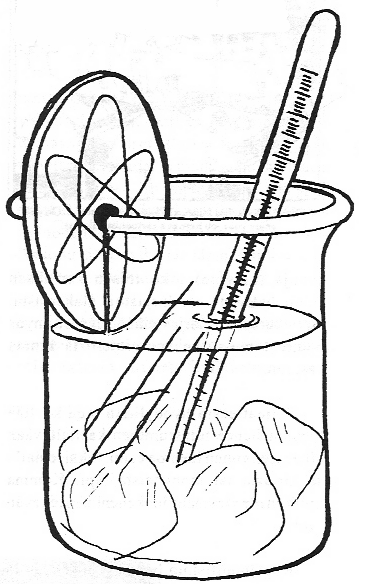
\includegraphics[width=\columnwidth]{cocktail.png}
	\end{figure}
	Se kuinka paljon luennoista saa irti,
	riippuu usein luennoitsijan lisäksi myös
	sinusta itsestäsi. Kaikkein hyödyllisintä on
	monen mielestä tutustua hieman etukäteen
	luennoilla käsiteltäviin aiheisiin, jolloin luennoitsijan
	ajatuksenjuoksun perässä pysyminen
	saattaa olla helpompaa. Luentomuistiinpanojen
	tekeminen kopioimalla kaiken
	mitä luennoitsija taululle tuhertaa (tai slaidilta
	lukee), ei välttämättä ole kovinkaan
	pitkälle järkevää. Pyrkimys tähän aiheuttaa
	useimmiten vain tylsistymistä, kynäkäden kramppia, sekä stressiä (varsinkin slaidit
	vaihtuvat välillä melkoista tahtia). Tämä on
	usein siinäkin mielessä turhaa, että useimmat
	luennoitsijat ovat tehneet valmiiksi tulostettavia
	prujuja ja luentorunkoja. Lisäksi
	Limes kustantaa kirjoja melkein kaikkiin
	fysiikan perus- ja aineopintojen kursseihin.
	Muistiinpanojen tekeminen reunahuomautuksiksi
	esimerkiksi prujujen reunoille, on
	mielestäni paljon järkevämpää (ja joskus
	kun väsymys painaa, se saattaa olla se asia,
	mikä pitää sinut liukumasta unen suloiseen
	huomaan).
	
	Luennolla kannatta aina kysyä, jos jokin
	asia esitetään epäselvästi. Todennäköistä
	on, että salissa on moni muukin ihmetellyt
	samaa asiaa. Opetushenkilökuntaa ei kannata
	pelätä, he ovat sinua varten, ja useimmiten
	oikeasti ihan mukaviakin.
	
	Fysiikan opiskelun pyhän kolmiyhteyden
	(luennot--laskarit--labrat) toinen kulmakivi
	vaatiikin jo sitten paljon luentoja
	enemmän työtä. Laskaritehtävät palautetaan viikoittain
	tarkastettaviksi joko netin välityksellä tai opetuslaboratorioiden
	aulasta löytyvään lokerikkoon.
	
	Laskareiden tekeminen vaatii aina
	enemmän aikaa kuin uskoisitkaan. Jos
	osaat lukion mekaniikan hyvin eikä matikkakaan
	tuota ongelmia, saattaa mekaniikan
	peruskurssin alkupään laskareista selvitä
	muutamassa tunnissa. Siitä eteenpäin niiden
	viemä aika vain kasvaa, teoreettisen
	fyssan laskarit voivat pahimmillaan olla
	koko viikon ja usean kymmenen sivun projekti.
	Laskareihin kannattaa siis varata reilusti
	suttupaperia.
	
	Mukavin tapa laskea laskareita
	on pieni ryhmä. Turhautumat eivät silloin
	pääse muodostumaan yhtä pitkäaikaisiksi,
	kun joku saattaa oivaltaa laskun perimmäisen
	salaisuuden ennen sinua. Mekaaninen
	kavereilta kopioiminen ei kuitenkaan ole
	järkevää, koska silloin ei opi asiaa; älä kangistu
	kaavoihin! Kannattaa liittyä suurin
	piirtein samantasoisten ihmisten seuraan
	laskemaan.
	
	Tenttiinkin on paljon mukavampi lukea
	jos ei ole pakko laskea sen toisen kurssin
	viimeisistä laskareista vähintään viittä todella
	vaikeaa tehtävää. Kannattaa sinnitellä
	alusta loppuun, keskimäärin kaksi oikein
	(tai sinne päin) ratkaistua tehtävää laskaria
	kohti riittää. Ylimääräisistä laskaripisteistä
	saa bonusta ainakin peruskursseilla, joten
	kannattaa laskea kaikki mitkä ehtii hyvän
	laskurutiinin saamiseksi.
	
	Opiskelun käytännönläheisimmästä
	osasta, labroista, on oma kuvauksensa
	muiden kurssikuvausten joukossa. Viisaita
	neuvoja ajankäytöstä ja muusta opiskelua
	tärkeämmästä löydät muualta tästä opuksesta.
	
	Muuten vielä yksi neuvo: ``Älä anna
	opiskelun viedä kaikkea aikaasi, elät juuri
	nyt todennäköisesti elämäsi parasta aikaa.
	Avaudu, älä eriydy. (Ja tämä ei siis tarkoita
	assareille avautumista)''.
	
	\twocolumn[\section{Tutkijapiiri}]
	Fysiikan osaston tutkijapiiri on opiskelijavetoinen ryhmä 
	tutkijanurasta haaveileville ja siitä mahdollisesti kiinnostuneille.
	Piirin ideana on tarjota sen jäsenille tietoa Fysiikan osastolla 
	tapahtuvasta tutkimuksesta erilaisten tapahtumien kautta. Tähän sisältyy
	siis erilaisia luentoja, teema\-tapahtumia, tiede\-retriitti ja joka kevät 
	järjestettävä kesä\-koulu. Tutkijapiiriin haku on vuoden\-vaihteen jälkeen 
	3.\,periodin aikana. Motivoitunut asenne ja into tutkimukseen on 
	tärkein haku\-kriteeri.
	
	\begin{figure}[b!]
		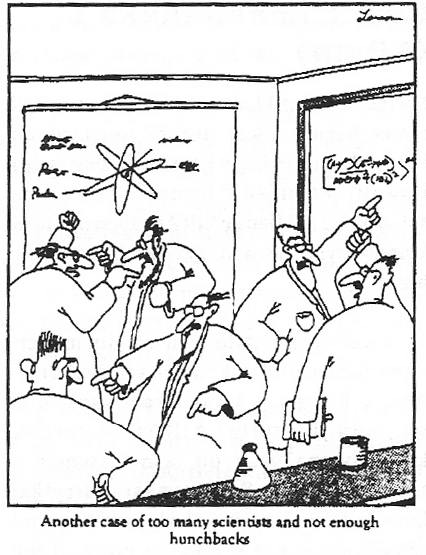
\includegraphics[width=0.8\columnwidth]{hunchback.png}
	\end{figure}
	Luennoilla eri alojen asian\-tuntijat tulevat kertomaan ajankohtaisista aiheista
	ja/tai omasta tutkimuksestaan. Aiheet vaihtelevat aina metalli\-vedystä 
	gravitaatio\-aaltoihin.
	
	Yksi teema\-tapahtumista on Fysikaalisiin tieteisiin perehtyminen "-kurssin 
	yhteydessä järjestettävä posteri\-sessio, jossa vanhemmat opiskelijat 
	pääsevät esittelemään postereitaan fukseille ja samalla tietenkin 
	harjoittelemaan niiden tekoa ja esittelyä. Välillä uskaltaudumme myös pois Physicumin turvasta ja käymme 
	tutustumassa myös muissa kohteissa tapahtuvaan tutkimukseen.
	
	Toukokuussa~2012 järjestettiin piirin ensimmäinen tiede\-retriitti ja 
	perinnettä on jatkettu; viimeisimmällä tiede\-retriitillä oltiin vuoden~2018 tammikuussa. Retriitissä toteutetaan pieniä tiede\-projekteja 
	pienissä ryhmissä tai yksin, joissa vain taivas (ja budjetti) ovat rajana. 
	Vanhoista projekteista mainittakoon vesi\-raketti ja sumu\-kammio-hiukkas\-ilmaisin.
	
	Lisäksi joka kevät touko\-kuussa tentti\-viikon jälkeen järjestetään noin viikon 
	kestävä kesäkoulu, joka on avoin kaikille fysikaalisten tieteiden opiskelijoille. 
	Aiheina aikaisempina vuosina on ollut esim.\,kosmologia, materiaali\-fysiikka, 
	hiukkas\-fysiikka ja tuoreimpana avaruus\-fysiikka.
	
	Tämän kaiken toiminnan lisäksi pääset tietenkin tutustumaan myös muihin piiriläisiin, johon erityisesti tiede\-retriitti tarjoaa loistavan mahdollisuuden. 
	Lisää infoa meistä löytyy tutkija\-piirin blogista \url{https://blogs.helsinki.fi/fys-tutkijapiiri/}.
	
	\vspace{0.5cm}
	\noindent\textsc{Anna Kormu}
	
	\twocolumn[\section{Fysiikan käytänteet}]
	\subsection*{Laskuharjoitukset}
	Laskuharjoitukset eli laskarit ovat osa
	lähes jokaista fysiikan kurssia.
	Laskarit ovat hyvä ellei jopa paras tapa
	oppia kurssin asiat. Toisin kuin luennoilla,
	laskareita tehdessä aktiivisena toimijana
	olet sinä. Vaikka lasku\-harjoitukset ovat toimiva
	oppimistapa, niitä on myös syytä tehdä
	siksi, että ne ovat pakollisia. Laskareista
	on yleensä saatava tietty määrä pisteitä, jotta
	sinulle myönnetään tentti\-oikeus. Yleensä
	määrä liikkuu kolmanneksen kieppeillä.
	Tämän lisäksi yleensä laskari\-pisteillä on
	myös vaikutusta kurssin loppu\-arvo\-sanaan
	noin kolmanneksen verran.
	
	\subsection*{Ilmoittautuminen laskuharjoituksiin}
	Pääasiassa peruskursseilla ilmoittaudutaan
	laskuharjoituksiin WebOodissa, mutta
	luennoijasta riippuen ilmoittautumiset saatetaan
	käytännössä hoitaa muinkin keinoin,
	esimerkiksi ensimmäisellä luennolla kiertävällä
	lapulla. Lasku\-harjoitus\-ryhmiä on
	tarjolla yleensä useampia. Kun kaikki ovat
	ilmoittautuneet, kurssin luennoitsijat järjestävät
	ryhmät järkevän kokoisiksi.
	
	Heidän työtään helpottaakseen on yleensä
	toivottavaa merkitä muutama sopiva
	ryhmä eikä pelkästään sitä, joka on kaikkein
	mieluisin. Tiedon omasta ryhmästä
	saa muutaman päivän kuluessa kurssin koti\-sivuilta
	tai seuraavalla luennolla. Kurssin
	koti\-sivuilta löytyvät myös laskari\-tehtävät.
	
	\subsection*{Laskareiden tekeminen ja palauttaminen}
	Laskareita kannattaisi alkaa tehdä heti,
	kun ne tulevat jakoon. Laskareiden tekoon
	on yleensä noin viikko aikaa, mutta viimeisenä
	iltana tehtäviä saa harvoin tehtyä
	kunnolla. Vähintäänkin laskemisesta oppii
	huomattavasti enemmän, jos niitä tekee
	rauhassa pitkin viikkoa. Tehtävät lasketaan
	ruutupaperille, jolla tehtävien lisäksi
	tulisi olla oma nimi, kurssin nimi, lasku\-harjoitusten
	numero sekä lasku\-harjoitusten
	aika ja niiden pitäjän eli lasku\-harjoitus\-assistentin
	nimi. Viimeiset tiedot tarvitaan,
	jotta paperit löytyvät myöhemmin oikeasta
	harjoitus\-ryhmästä. Myös opiskelija\-numeron
	kirjoittaminen on suotavaa, sillä sitä
	käytetään kurssin tulosten kirjaamiseen ja
	ilmoittamiseen.
	
	Viime vuosina myös netin kautta tapahtuva laskari\-palautus on yleistynyt peruskursseilla. Tällöin laskari\-paperista skannattu tai kameralla otettu (hyvä\-laatuinen) kuva palautetaan kurssin Moodle-alueelle. Toki laskarit voi latoa suoraan \texttt{pdf}-tiedostoksi käyttämällä vaikkapa {\LaTeX}ia (jolla tämäkin kirja on tehty).
	
	Laskareiden tekemisessä ryhmä\-työskentely on
	täysin hyväksyttävää ja todella suositeltavaa.
	Ryhmästä saa ajatuksia, joiden keksimiseen
	saattaisi yksin mennä iäisyys. Laskareita
	saattaa kuitenkin kannattaa tutkia
	ensin myös yksin, jottei ryhmä\-työ mene
	pelkäksi kopioimiseksi, joka taas kostautuu
	myöhemmin tentissä. Koska kukaan ei voi
	kertoa toiselle juuri hänelle parhaiten sopivaa
	metodia, jokaisen on löydettävä itse
	oma tapansa.
	
	Useimmilla perus\-kursseilla lasku\-harjoitus\-tilaisuudet ovat ennen lasku\-harjoituksien palauttamista. Tällöin laskari\-tilaisuuksissa on tarkoitus pohtia viikon laskari\-tehtäviä assarin avustuksella. Laskari\-tilaisuudet ovat mitä mainioin paikka löytää lasku\-seuraa, jos yksin puurtaminen alkaa kyllästyttämään. On sallittua myös käydä useammassa laskari\-tilaisuudessa, jos tuntee kaipaavansa vielä lisää vinkkejä laskuihin. Joillakin kursseilla lasku\-harjoitukset täytyy palauttaa
	etukäteen tarkastettavaksi. Tällöin laskari\-tilaisuuksissa käydään läpi palautettujen tehtävien malli\-ratkaisut.
	
	Ellei kurssilla ole käytössä sähköistä palautusta, laskarit palautetaan
	lähes poikkeuksetta 2.\,kerroksen
	A-siiven (opetus\-laboratoriot) aulassa oleviin
	lokerikkoihin. Palautettaessa irralliset
	paperit täytyy liittää yhteen. Viimeinen
	palautus\-aika kerrotaan ensimmäisillä luennoilla ja kurssin koti\-sivuilla. Palautus\-aikaa
	kannattaa noudattaa, sillä on parempi saada
	pisteet muutamasta tehtävästä kuin ottaa
	riski, että assistentti (eli assari) ei enää ota
	paperiasi etkä saa yhtään pistettä.
	
	Joillain kursseilla on käytössä matemaattisten tieteiden suosima tyyli, jonka
	mukaan etukäteen tehdyt tehtävät otetaan
	mukaan laskari\-tilaisuuteen. Tilaisuuden
	alussa merkitään paperiin mitä tehtäviä on
	tehty, ja merkintöjen perusteella jaetaan
	pisteet. Laskareiden aikana assari valikoi
	listalta merkintöjen perusteella henkilöt,
	jotka tekevät malli\-vastaukset taululle. Näitä
	``rasti ruutuun "-laskareita'' on ollut viime vuosina
	myös fysiikan perus\-kursseilla, mutta silti
	yleisempiä ovat palautettavat laskarit.
	
	\subsection*{Laskareissa käyminen}
	Lasku\-harjoituksissa käyminen on vapaa\-ehtoista
	useimmilla fysiikan perus\-opintojen kursseilla. Laskareissa kannattaa
	kuitenkin käydä, jos kaikki viikon tehtävät eivät ole aivan päivän\-selviä. Assarin antamien vinkkien avulla pystyy välttämään pahimmat umpikujat ja saamaan idean miten kutakin tehtävää kannattaa aloittaa ratkaisemaan. Assarilta voi myös tarkistaa onko oma ratkaisu\-yritys mennyt oikein ja kysyä selvennystä, jos jokin viime viikon laskareissa tai luennoissa on jäänyt epäselväksi. Joillain kursseilla saa myös
	lisä\-pisteitä käymällä laskareissa ja esittämällä
	oman ratkaisunsa.
	
	\subsection*{Lisähuomio aineopinto- ja syventävistä kursseista}
	Lopuksi on todettava, että tässä esitetty
	ei välttämättä päde myöhempien opintojen
	(aine\-opinnot ja syventävät opinnot)
	kursseihin. Niissä varsinkin syventävillä
	kursseilla lasku\-harjoitukset saattavat olla
	kokonaan vapaa\-ehtoisia ja laskareista saatava
	hyöty saattaa vaihdella paljon. Kunkin
	kurssin käytännöt selviävät kuitenkin aina
	viimeistään kurssin ensimmäisillä luennoilla.
	
	\vspace{0.5cm}
	\noindent\textsc{Pentti Arffman}\\
	\textsc{Joonas Herranen}\\
	\textsc{Antti Pirttikoski}
	
	\twocolumn[\section{Kursseja, kursseja, kursseja}]
	\subsection*{Fysiikan perusopinnot}
	Fysikaalisten tieteiden kandiohjelman opiskelijat suorittavat
	fysiikan perusopinnot käymällä neljä luentokurssia
	ja laboratoriokurssin. Kaikilla
	luento\-kursseilla viikko-ohjelma on melko
	samanlainen. Luentoja on noin neljä tuntia,
	laskareita kaksi tuntia sekä mahdollisesti
	lasku\-paja\-päivystystä kaksi tuntia. Lasku\-paja\-päivystyksessä
	assistentti neuvoo lasku\-harjoitusten
	tekemisessä. Silloin tällöin
	luentojen lomassa on myös demonstraatioita,
	joissa yritetään vaihtelevalla menestyksellä
	havainnollistaa fysiikan lakeja.
	
	Labratöiden ohjelma seuraa luentojen
	aihepiiriä. Laboratorio\-töitä tehdään viikossa
	kaksi tuntia. Työvuoroilla käydään
	tekemässä samoja kokeita, joita jo tuhannet
	opiskelijat ovat tehneet. Silti tulokset ovat
	ajoittain uusia, jopa yllätyksellisiä! Vuoden
	aikana tehdään yhteensä 12~laboratoriotyötä,
	joista jokaisesta kirjoitetaan raportti.
	Perus\-opintojen laboratorio\-töissä raportin
	pituus on noin viisi sivua (kuvien kera).
	
	Laskareista on yleensä laskettava kolmas\-osa,
	jos aikoo selviytyä läpi. Toki kannattaa
	laskea niin paljon kuin osaa ja ehtii,
	koska laskareista saa hyvin bonus\-pisteitä
	koe\-pisteiden jatkoksi, ja jokainen tehtävä
	kartuttaa asian ymmärrystä. Lisäksi kokeissa
	on usein laskareista tuttuja tehtäviä.
	Arvosteluasteikko perus\-kursseilla on ollut
	suhteellisen löysä. Perus\-kursseilla on siirrytty kokonaan sähköiseen palautukseen, jossa laskarit palautetaan suoraan kurssin Moodle-sivuille.
	
	Palautus\-ajoissa kannattaa olla
	tarkka, sillä kaikki assistentit eivät suostu
	ottamaan tarkastettavaksi myöhässä palautettuja papereita. Kannattaa muistaa, että
	kaikki muut fysiikan opinnot pohjautuvat
	peruskurssien tiedoille ja siksi niihin kannattaa
	panostaa. Hyvin suoritettujen perus\-kurssien
	jälkeen monet muut kurssit saattavat
	tuntua helpoilta.
	
	\vspace{0.5cm}
	\noindent\textsc{Joonas Herranen}
	\subsubsection*{Vuorovaikutukset ja kappaleet (5~op)}
	Fysiikan suossa tarpominen on jo muinaisista
	ajoista asti aloitettu mekaniikan
	opinnoilla, joten syksyn ensimmäisessä
	periodissa luennoitava Vuoro\-vaikutukset
	ja kappaleet on mitä suositeltavimpia
	fuksi\-kursseja. Kurssin aikana Newtonin
	mekaniikka ja erilaiset vuorovaikutukset
	tulevat tutuksi lukiota hieman matemaattisemman
	formalismin kautta. Mitään demonisia
	integraaleja tai derivaattoja ei ole
	odotettavissa, joten matemaattisesti sekä
	fysikaalisesti lukion pitkien aineiden jälkeen
	kurssin kunnialliseen suorittamiseen
	vaaditaan lähinnä tasaista puurtamista ja
	valmiutta piirrellä vektoreita. Lisä\-apua
	kurssin suorittamiseen voi hakea matematiikan
	opinnoista (Maput tai
	matematiikan fuksikurssit).
	
	\subsubsection*{Vuorovaikutukset ja aine (5~op)}
	Fuksi\-syksy jatkuu toisessa periodissa
	luennoitavalla kurssilla Vuoro\-vaikutukset
	ja aine, jonka aikana harjoitellaan mallintamaan
	reaali\-maailman systeemejä formalismilla,
	joka on myös opintojen myöhemmissä
	vaiheissa käyttö\-kelpoinen. Kurssilla tutustutaan
	pyörimis\-liikkeeseen, energian kvantittumiseen
	ja niin monen hiukkasen systeemeihin,
	että jouluun mennessä tunnetaan
	kineettisen kaasuteorian ja entropiankin
	alkeita. Jos koet eläväsi kolmi\-ulotteisessa
	maailmassa, ei kurssin aikana pitäisi tulla
	vastaan perustavanlaatuisia haasteita.
	
	\vspace{0.5cm}
	\noindent\textsc{Joonas Herranen}
	\subsubsection*{Perusopintojen laboratoriotyöt (5~op)}
	Fysiikan perus\-kursseihin kuuluu vuoden
	aikana käytävä kokoelma laboratorio\-töitä,
	joita on aika\-taulutettu jokaiselle yksittäiselle
	kurssille kolme kappaletta. Laboratorioissa
	tutustutaan perus\-kurssien luentojen
	aikana tutuiksi tulleisiin aiheisiin erinäisten
	kokeiden ja mittausten avulla, joten on suositeltavaa suorittaa nämä muiden peruskurssien
	kanssa samanaikaisesti.
	Labroissa kulutetaan yleensä pari--kolme
	tuntia viikottain muutaman hengen
	ryhmissä, joskin jokaista labraa ennen on
	suunniteltava työn kulku ja saatava mainiolle
	suunnitelmalleen vihreää valoa
	näyttävä assari (ei mitenkään mahdoton
	työ, sillä tarvittavat laboratorio\-laitteet ovat
 yhtä monimutkaisia kuin rauta\-lanka).
	Töistä laaditaan raportti, josta käy
	ilmi työssä välttämätön teoria, mittauksen
	yksityiskohdat, tulokset virhe\-arvioineen ja
	johto\-päätökset, eli kuinka hyvin mittaukset
	vastasivat teoriaa.
	
	Kurssin suoritus, lähinnä raporttien
	oikeaoppinen laatiminen, vaatii hieman
	oma\-toimista opiskelua tai läsnä\-oloa syksyn
	luennoilla, mutta muuten labrojen vaatimukset
	ja tahti ovat varsin rentoja. Ja mikäpä
	on hauskempaa kuin rauta\-kuulan ampuminen
	ensi\-yrittämällä ämpäriin, kun on
	ensin laskenut ammuksen osumakohdan paperilla!
	
	\vspace{0.5cm}
	\noindent\textsc{Joonas Herranen}
	
	\subsubsection*{Sähkömagnetismi (5~op)}
	Kurssilla tutustutaan sähkö\-statiikan perusteisiin
	ja ilmiöihin sekä materiaalien
	sähköisiin ja magneettisiin ominaisuuksiin. Kurssiin kannattaa panostaa
	silmällä pitäen seuraavan periodin
	Säteily\-kentät ja fotonit "-kurssia, jossa sähkö\-magnetismissa
	opittuja tietoja päästään
	soveltamaan. Tässä kohtaa päästään myös hyödyntämään MaPulla opittuja integroimis\-taitoja
	tositoimissa.
	
	\vspace{0.5cm}
	\noindent\textsc{Joona Havukainen}
	
	\subsubsection*{Säteilykentät ja fotonit (5~op)}
	Tämä kurssi jatkaa siitä mihin sähkö\-magnetismissa
	jäädään. Maxwellin yhtälöiden
	johtaminen ja soveltaminen, kiihdyttelevien
	varauksien synnyttämät sähkökentät
	sekä valon sironta ja käytös väliaineen
	kanssa ovat tämän kurssin ydinasiaa. Kurssi
	tarjotaan toisessa ja neljännessä periodissa,
	ja SäFo kannattaa käydä yhtenä jatkumona
	sähkömagnetismin kurssin kanssa. Luonnollisesti
	Mapun taidot pääsevät tässäkin
	kurssissa oikeuksiinsa, ja Sähkö\-magnetismin
	kurssin asioiden hyvä hallinta antaa
	vahvan pohjan SäFoa varten.
	
	\vspace{0.5cm}
	\noindent\textsc{Joona Havukainen}
	
	\subsection*{Matemaattisten ja laskennallisten menetelmien kokonaisuus}
	\subsubsection*{Matemaattiset apuneuvot I--III (5+5+5~op)}
	Matemaattisia apuneuvoja
	suositellaan kaikille fysiikkaa opiskeleville
	heti ensimmäisenä syksynä. Kurssilla
	käydään läpi kaikki fysiikan perus\-kursseilla
	käytävä matematiikka ja on melko laaja. Tästä huolimatta kurssit eivät
	ole mitenkään mahdottomia ja ne sujuvat
	kyllä hyvin, jos viitsii uurastaa. Mapujen
	asioiden hallitseminen on myös edellytys
	myöhemmillä fysiikan kursseilla pärjäämiseksi.
	Esi\-tietoina lukion pitkä matematiikka
	on riittävä. Jos tätä ei ole kuitenkaan tullut
	käytyä tai olo on muuten epävarma, voi
	olla järkevää käydä myös joitain perus\-kursseja
	matemaattisten tieteiden kandiohjelmasta.
	
	Pieni varoituksen sana matematiikan opinnoista lienee kuitenkin paikallaan.
	Kun matematiikan laitos lopetti
	kurssien Approbatur I--II luennoimisen
	loppuivat matematiikalta käytännölliseen
	matematiikkaan suuntautuneet
	kurssit lähes kokonaan. Parhaiten näihin
	asioihin päässee sisälle analyysin peruskursseilla tai Samuli Siltasen \textsc{Matlab}-kursseilla. Vektori\-laskentaa ja
	matriiseja käsittelevään osuuteen kannattaa
	tutustua kurssilla Lineaari\-algebra ja matriisi\-laskenta~I (5~op), vektori\-avaruuksia käsittelevään
	taas tämän kakkos\-osalla (myöskin
	5~op). Toisaalta käyrä-, pinta-ala- ja tilavuus\-integrointi
	tulee vasta Vektorianalyyseillä
	(5+5~op).
	
	\subsubsection*{Tieteellinen laskenta~I (5~op)}
	Tieteellinen laskenta~I "-kurssilla opetellaan
	Linux/Unixin käytön perusteet, opetellaan
	labra\-selkkareissa ja muissa kirjoitelmissa
	erittäin hyödyllisen ladontakielen
	{\LaTeX}in käyttöä sekä opetellaan ohjelmoinnin
	alkeita Pythonilla.
	Kurssi pidetään syksyllä toisessa periodissa. Kurssi ei edellytä esitietoja,
	joskin ohjelmoinnin perusteista on
	varmasti iloa. Kurssilla on melko paljon
	asiaa, joten yksittäisiin aihe\-piireihin ei ehditä
	paneutua kovinkaan syvällisesti. Jos
	haluat perehtyä tarkemmin erityisesti kurssin
	ohjelmointi\-puoleen, on ohjelmoinnin
	perusteet tietojen\-käsittely\-tieteen puolelta
	erinomainen lisä joko ennen kurssia tai sen
	jälkeen.
	
	\subsubsection*{Havaintojen tilastollinen käsittely (5~op)}
	HaTiKällä, TiHalla tai HTK:lla käydään läpi kaikille fyysikoille
	tarpeellisia tilastomenetelmiä. Tilastolliset
	tunnusluvut, todennäköisyysjakaumat,
	tilastollinen estimointi ja testaus tulevat täällä
	tutuiksi. Aivan kurssin loppuvaiheessa sivutaan myös kaaosteoriaa ja Fourier-analyysiä. 
	
	Osa kurssin laskareista tehdään valmiilla Python-skripteillä, joita pitää muokata vain hieman. Muuten tehtävät eivät ole erityisen vaikeita, mutta niissä kyllä itse kukin pääsee nyrjäyttämään aivonsa ympäri ja leikkimään oikeaa tilastotieteilijää.
	\subsection*{Fysiikan aineopintoja}
	\subsubsection*{Termofysiikan perusteet (5~op)}
	Kurssin sisältö käsittää klassisen termofysiikan. Luennoilla opitaan muun muassa mitä työllä ja energialla on tekemistä keskenään ja miksi Reino on
	huono tuho\-polttaja.
	
	Matemaattisesti kurssi ei ole erityisen
	raskas, mutta kuten aina, MaPut kannattaa
	olla käytynä. Kursseilla on yleensä käytetty
	laadukasta luento\-prujua materiaalina.
	
	\subsubsection*{Termodynaamiset potentiaalit (5~op)}
	Kurssi käsittelee Maxwellin relaatiot ja vapaat energiat. Lisäksi kurssilla suunnitellaan ja kirjoitetaan
	oma pieni tutkielma jostain termo\-fysiikan
	aiheesta.
	
	Yleensä TerPe ja TerPot käydään toisen vuoden
	syksynä, kun differentiaaliyhtälöihin on jo
	törmätty muilla kursseilla. Kursseista on
	hyötyä myöhemmin ainakin statistisella
	fysiikalla ja etenkin meteorologit käyttävät
	kurssin oppeja väistämättä tulevissa opinnoissaan. Tähtitieteilijöille termot eivät ole pakollisia, vaan he korvaavat tutkielman Kerro tähtitieteestä "-kurssilla. 
	
	\subsubsection*{Kvanttifysiikan perusteet (5~op)}
	Fuksin ensipuraisu kvantti\-mekaniikan
	tavanomaista intuitiota uhmaavaan maailmaan.
	Kurssilla tutustutaan hieman fysiikan
	historiaan ja käänteisiin, jotka johtivat
	kvanttimekaniikan syntyyn, Schrödingerin
	yhtälön pyörittelyyn ainakin laatikkoon
	vangitun hiukkasen tapauksessa sekä muihin
	kvantti\-mekaniikan perusilmiöihin, kuten
	tunneloitumiseen.
	
	Kurssi järjestetään kolmos\-periodissa ja se toimii SuPerin kanssa yhdessä katsauksena
	modernin fysiikan maailmaan.
	
	\subsubsection*{Kvanttifysiikan sovelluksia~I -- Atomit ja molekyylit (5~op)}
	Tällä kurssilla siirrytään kvanttifysiikan
	perusteista yksinkertaisimpien atomien ja
	molekyylien maailmaan, jossa ovelat approksimaatiot
	tuottavat kaikkien käytännön
	sääntöjen mukaan lähes koko lukio\-kemian.
	Kurssilla siis tutustutaan peruskursseilla
	tutuiksi tulleisiin yhtälöihin pall\-okoordinaateissa
	ja yritetään saada niistä jotain
	fysikaalisesti järkevää ulos myös tilanteissa,
	joissa on useampi kuin kaksi hiukkasta
	kyseessä.
	
	\subsubsection*{Kvanttifysiikan sovelluksia~II -- Tiivis aine ja alkeishiukkaset (5~op)}
	Jos vanhemmat puhuvat kurssista nimeltä
	Aineen rakenne, puhuvat he hyvin luultavasti
	tämän kurssin sisällöistä.
	Nykyisin Kvantti\-fysiikan sovelluksia~II pitää sisällään
	karkeahkosti arvioitua kvantti\-fysiikkaa, ja
	tämän avulla päästään käsiksi mm.\,metallien
	sähkönjohtavuuden selittämiseen, josta
	siirrytään puoli\-johteitten merkilliseen maailmaan.
	Ydinreaktioiden käsittelyn jälkeen
	tutustutaan hiukkas\-fysiikkaan ja lopuksi
	käsitellään vielä atomin pienimpiä rakenne\-osasia.
	
	\subsubsection*{Fysiikan mittausmenetelmät (5~op)}
	Fysiikan mittaus\-menetelmät lukeutuu
	fysiikan aine\-opintojen pakollisiin kursseihin
	ja sen sopiva suoritus\-ajan\-kohta on toisen
	vuoden syksyllä.
	
	Koska fysiikka on pohjimmiltaan kokeellinen
	tiede, on kurssi hyödyllinen myös
	kaikille sivu\-tieteen\-ala\-opiskelijoille.
	Kurssi ei ole etenkään
	matemaattisesti kovin haastava, mutta lukuisten
	uusien käsitteiden sisäistämisessä saattaa hurahtaa muutama tovi. Pohja\-tietona
	Fysiikan perus\-opinnot ovat enemmän
	kuin riittävät.
	
	Kurssilla käydään läpi yleisimpiä mitta\-laitteita
	ja "-järjestelmiä, tulosten tilastollista
	käsittelyä ja mittaus\-elektroniikan perusteita.
	Kurssilla selviää muun muassa, mitä
	eroa on valkoisella, harmaalla, ruskealla ja
	pinkillä kohinalla. Jos aikaa jää, loppuosalla
	kurssia perehdytään tarkemmin elektroniikan
	perusteisiin, ja sopiva jatkokurssi onkin
	syksyn toisessa periodissa luennoitava
	Elektroniikka~I.
	
	Kurssin lasku\-harjoituksilla on melko
	suuri paino\-arvo ja harjoitus\-tilaisuuksissa
	esitettävistä demoista saa ilmaisia lisäpisteitä,
	joten tehtäviä kannattaa tehdä ja käydä
	tarkistamassa niin paljon kuin mahdollista.
	
	\subsubsection*{Fysiikan aineopintojen laboratoriotyöt~I--II (5+5~op)}
	Aineopintojen laboratorio\-työt on nykyisessä
	tutkinto\-rakenteessa jaettu kahteen eri
	kurssiin. Kurssit suoritetaan tekemällä
	assistenttien järjestämien neli\-tuntisten
	työ\-vuorojen aikana kolme työtä molempia kursseja kohden, jotka liittyvät
	aihe\-piireiltään muun muassa termo\-fysiikkaan, elektroniikkaan
	sekä atomi- ja ydin\-fysiikkaan. Töistä
	palautetaan aina kirjalliset selostukset/
	raportit.
	
	Aine\-labroihin sisältyy myös lasku\-harjoituksia, joissa tutustutaan etukäteen kunkin viikon työn aihe\-piiriin ja data-analyysissä tarvittaviin menetelmiin.
	Labratöiden vaativuus, laajuus ja kesto
	vaihtelevat melko paljon, kunkin työn
	helppous ja mukavuus on paljolti kiinni
	niin omasta itsestä, assistentista kuin Murphyn
	lain hetkellisestä voimakkuudestakin.
	
	Kunkin työn ohjeet on syytä lukea ajatuksella
	ennen työ\-vuoroa, joissain jopa
	kehotetaan lukemaan tai laskemaan asioita
	etukäteen. Toisin kuin perus\-opinnoissa,
	työt suoritetaan itsenäisesti ja omiakin
	aivoja joutuu käyttämään (sen sijaan, että
	kuolaisi vaan krapulassa, kun kaverit hoitavat
	homman kotiin). 
	
	Kaikista labra\-töistä kirjoitetaan
	selostus sisältäen tiivistelmän, johdannon,
	teoria\-osuuden, kuvauksen mitta\-laitteistosta
	ja mittauksista, tulokset ja (viimeisenä, muttei todellakaan vähäisimpänä) johto\-päätökset.
	Loppuun tulevat tietenkin vielä
	lähde\-luettelo sekä liitteet, joiden työn luonteesta
	riippuva määrä on käytännössä ehkä
	eniten paperi\-nipun paksuuteen vaikuttava
	tekijä.
	
	\subsubsection*{Tieteellinen laskenta~II (5~op)}
	Tieteellinen laskenta~II keskittyy lähinnä
	tieteellisessä laskennassa käytettävän
	Fortran-kielen opetteluun, joskin kurssin
	laskarit pystynee suorittamaan kysyttäessä myös C- tai C++ "-kielillä, joita ei kuitenkaan
	kurssilla opeteta. Kurssi järjestetään
	syksyisin ja se on kahden periodin mittainen.
	Ohjelmoinnin perusteista on varmasti
	paljon iloa tällä kurssilla, joskin kurssi on
	mahdollista käydä ilmankin, mikä tosin
	vaatii aika paljon enemmän työskentelyä
	laskarien parissa.
	
	Laskarien vaikeustaso riippuu hyvin
	paljolti aikaisemmasta ohjelmointi\-kokemuksesta.
	Paljon ohjelmoinut selviää
	kurssista huomattavasti pienemmällä työmäärällä
	kuin esimerkiksi pelkästään Tieteellinen
	laskenta~I:n käynyt.
	
	Kurssilla on melko paljon lasku\-paja\-päivystystä
	jossa kannattaa käydä erityisesti
	jos aikaisempaa ohjelmointi\-kokemusta
	on vähän. Epä\-selvyyksiin saa usein
	vastauksia joko assareilta tai luennoitsijalta
	kurssin Moodle-sivun keskustelu\-alueelta,
	joskus yllättävänkin nopeasti.
	
	\subsubsection*{Fysikaalisiin tieteisiin perehtyminen (3~op)}
	Syys\-lukukauden aikana esitellään fysikaalisia
	tieteitä ja niiden tutkimus\-kohteita.
	Kurssista pääsee läpi kunhan on läsnä
	tarpeeksi monella luennolla; noin kolme
	poissa\-oloa sallitaan. Luennoista täytyy kirjoittaa
	myös referaatteja, jotka palautetaan
	luennoitsijalle tiettyyn määrä\-aikaan
	mennessä. Luennoilla kannattaa käydä, sillä
	näin saa edes hieman kuvaa siitä kuinka
	laajan alueen fysiikka kattaa. Kurssilla pääsee myös haastattelemaan työelämässä olevia fyysikoita joillakin luento\-kerroilla. 
	
	\subsubsection*{Naturvetenskap nu I--II (2+2~op)}
	Läsnäolopakollinen luento\-kurssi, jossa käy luennoitsijoita laajasti Kumpulan eri tutkimusaloilta puhumassa mielenkiintoisista aiheista. Vuonna 2017 luennoilla oli usein sämpylä- ja viini\-tarjoilut, ja kurssi päättyi sitseihin. Kurssi on ruotsinkielinen, mutta ei edellytä hyvää ruotsin kielen taitoa. (Tällä ei kuitenkaan valitettavasti voi korvata pakollista ruotsinkurssia.)
	
	\subsection*{Teoreettinen fysiikka}
	\subsubsection*{Suhteellisuusteorian perusteet (5~op)}
	Kurssilla esitetään suppea suhteellisuus\-teoria
	ja siihen perehdytään sitten kunnolla.
	Monet kyllä törmäävät suhteellisuus\-teoriaan
	tämän kurssin jälkeenkin, mutta näin
	perusteellisesti sitä ei enää myöhemmin
	käydä.
	
	Kellot ja koordinaatistot ehtivät saada
	kyytiä moneen kertaan selviteltäessä
	avaruusalusten keskinäistä sijaintia niiden
	matkatessa läpi neljän ulottuvuuden. Samalla
	löytyy syy myös sille, miksi nopeasti
	liikkuvan kohteen säteilemän valon aallon\-pituus
	muuttuu. Kun suppeamman suhteellisuus\-teorian
	käsitteet ovat tulleet tutuiksi,
	tutustutaan lopuksi vielä yleiseen suhteellisuusteoriaan
	ja sen mukanaan tuomiin ilmiöihin,
	kuten gravitaatio\-aaltoihin ja avaruuden
	kaareutumiseen, jonka avulla voidaan
	selittää mustien aukkojen olemassaolo.
	
	\begin{figure}[]
		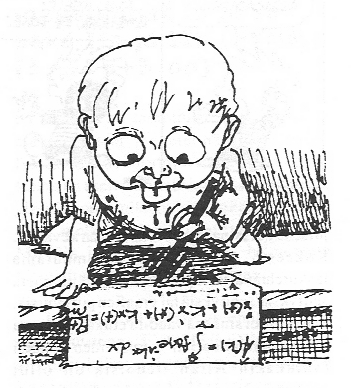
\includegraphics[width=\columnwidth]{teorfys_vauva.png}
	\end{figure}
	
	Kurssi on ajatus\-maailmaltaan monelle
	hankala, ja henkilöstä riippuen laskarit joko
	menevät täysin yli hilseen tai sitten vaativat
	vähintään pään\-vaivaa. Huumori on perinteisesti
	ollut vahvasti läsnä laskari\-tehtävissä.
	
	\subsubsection*{Kvanttifysiikan perusteet (5~op)}
	Fuksin ensipuraisu kvantti\-mekaniikan
	tavanomaista intuitiota uhmaavaan maailmaan.
	Kurssilla tutustutaan hieman fysiikan
	historiaan ja käänteisiin, jotka johtivat
	kvantti\-mekaniikan syntyyn, Schrödingerin
	yhtälön pyörittelyyn ainakin laatikkoon
	vangitun hiukkasen tapauksessa. Kurssi järjestetään
	kolmosperiodissa ja se toimii SuPerin
	kanssa yhdessä katsauksena modernin
	fysiikan maailmaan. 
	
	\subsubsection*{Analyyttinen mekaniikka (5~op)}
	Analyyttinen mekaniikka (kutistettu entisestä
	Klassisesta mekaniikasta) on pakollinen
	teoreettisen fysiikan aine\-opinto\-kurssi.
	Teoreettisen fysiikan opiskelijat käyvät sen perinteisesti
	toisena opiskelu\-vuonna. Esitietoina edellytetään
	Mapuja ja fysiikan perus\-opintoja.
	
	Kurssi tarjoaa kaksi erilaista, tapaa lähestyä
	klassista mekaniikkaa: Lagrangen ja Hamiltonin formalismin.
	Nämä ovat täysin ekvivalentteja Newtonin
	formalismin kanssa, jossa liike\-yhtälöt muodostetaan
	voimien avulla.
	
	Lagrangen ja Hamiltonin formalismit
	toimivat liike- ja potentiaali\-energioiden
	pohjalta. Kurssilla syvennytään myös pyörimis\-liikkeen
	ja värähtelijöiden ongelmiin
	huomattavan paljon peruskursseja raskaammalla
	kalustolla.
	
	Erityisesti Hamiltonin formalismin kieroudet
	kannattaa opetella kerralla kunnolla,
	sillä myöhemmin kvantti\-mekaniikan matemaattisen
	formalismin ymmärtäminen
	helpottuu niiden välisten yllättävien yhtäläisyyksien
	vuoksi.
	
	Kurssi on perus\-opintojen vastaavia kursseja
	huomattavasti teoreettisempi ja yltyy
	laskennallisesti paikoin hyvinkin raskaaksi,
	jolloin laskareiden tekoon ja aiheen opetteluun
	kannattaa varata huolella aikaa. Kurssikirjaksi
	sopii hyvin Koskisen--Vainion
	Klassinen mekaniikka, joka on tehty kurssin
	samannimisen edeltäjän luentojen pohjalta.
	Myös Landaun--Lifšitsin kirjasarjan ensimmäinen opus on tutustumisen arvoinen.
	
	\subsubsection*{Statistinen mekaniikka (5~op)}
	Statistinen mekaniikka, tutummin StaMek,
	käydään perinteisesti viimeisenä teoreettisen
	fysiikan aine\-opinnoista. Fysikaalisten tieteiden opiskelijoille
	tämä ajoittuu kolmannen vuoden
	keväälle. Kurssi lähestyy termo\-fysiikan ongelmia
	toisesta näkökulmasta. Kurssin suorittaminen
	edellyttää hyvää termo\-fysiikan hallintaa,
	jonkin tasoista kvantti\-mekaniikan tuntemusta,
	klassisen mekaniikan Hamiltonin
	formalismin tuntemista ja FYMM~Ib:n matemaattisen
	työ\-kalu\-pakin osaamista.
	
	Kurssi alkaa klassisella faasi\-avaruuden
	käsittelyllä, jossa otetaan käyttöön termi
	tila\-tiheys. Tästä siirrytään kvantti\-mekaniikkaan
	ja diskreetteihin energia\-väleihin,
	jotka silti approksimoidaan usein jatkuviksi.
	Tärkeimpinä suureina esitellään erilaiset
	tila\-summat, joista kaikki systeemin tilastolliset
	ominaisuudet voidaan laskea.
	Kurssin loppupuolella käsitellään bosonien
	ja fermionien statistiikkaa ja erilaisia
	faasi\-transitioita.
	
	Kurssikirjana käytetty Arposen--Honkosen
	Statistinen fysiikka "-kirja on kurssilla
	hyödyllinen, joskin itse\-opiskeluun se ei
	sovellu ja kirjasta oppii heikosti varsinaista
	fysiikkaa. Kurssilla oppii raskaiden laskareiden
	kanssa päätä seinään hakatessa luovia
	laskenta\-tapoja ja approksimaatio\-kikkoja.
	
	\subsubsection*{Elektrodynamiikka~I+II (5+5~op)}
	Elektrodynamiikan ``kiehtovaan'' maailmaan
	aloitteleva teoreetikko tipahtaa
	yleensä toisena opiskelu\-vuotenaan, fyysikot
	ehkä myöhemmin, jos silloinkaan.
	Elektro\-dynamiikka, kavereiden kesken
	ED, on teoreettisen fysiikan aine\-opintojen
	kurssi, jonka voi myös sisällyttää halutessaan
	fysiikan syventäviin opintoihin.
	
	ED on tyypillinen teoreettisen fysiikan
	aine\-opintojen kurssi, josta selviää kunnialla
	tekemällä ahkerasti töitä ja laskareita.
	Laskarit saattavat tuntua (luennoitsijasta
	riippuen) välillä jopa liian lasku\-teknisiltä,
	mutta osaapahan kurssin jälkeen ainakin
	derivoida vektoreita (muista derivointi karteesisessa
	koordinaatistossa)!
	
	Kurssi alkaa jo aiemmilta kursseilta tutulla
	Coulombin lailla ja päättyy hirviöön,
	joka kuvaa yleisessä liikkeessä olevaa varattua
	hiukkasta. Välivaiheet kannattaa
	usein lukea esimerkiksi Griffithsin kirjasta.
	Luennoitsijasta riippuen myös suhteellisuusteoriaa
	ja plasmafysiikkaa voi kurssin
	loppu puolella vilahdella.
	
	ED:llä mekaaninen laskutaito on valttia.
	Esitietona kurssille vaaditaan FYMM~I, ja
	FYMM~II tulisi suorittaa viimeistään yhtä
	aikaa ED:n kanssa. Tietysti myös MAPU~I--III
	tulisi olla hallinnassa, sillä ED:llä
	joutuu tahi pääsee niiltä tuttuja taitoja oikeasti
	soveltamaan. Apua kurssin alkupuolella
	on myös sähkömagnetismin peruskurssien hallinnasta.
	
	Kurssin aihepiiriin liittyvää kirjallisuutta löytyy kirjastosta metreittäin, mutta D.~J.~Griffithsin ``Introduction to Electrodynamics''
	lienee parhain, jos ei halua intohimoisesti
	kahlata läpi J.~D.~Jacksonin ``Classical
	Electrodynamics'' "-raamattua lävitse.
	Muista mahdollisesti hyödyllisistä kirjoista
	mainittakoon Reitz--Milford--Christyn
	``Foundations of Electromagnetic theory'',
	Cronström--Lippaan suomenkielinen ``Johdatus
	sähködynamiikkaan ja suhteellisuusteoriaan'',
	sekä tietysti Landaun klassikot.
	
	Luentoprujut ovat printattavissa suomen\-kielisinä
	kurssin kotisivulta. Prujut kattavat
	kaikki kurssilla käsitellyt asiat, mutta
	laskuesimerkkejä mielellään etsii oheis\-lukemistosta.
	Prujujen lukeminen kuitenkin
	kannattaa, sillä yleensä välikokeeseen tulee
	yksi johtotehtävä lähes suoraan niistä.
	
	ED:n asiat kannattaa ehdottomasti opetella
	hyvin, jos jatkossa haluaa välttää turhaa
	pähkäilyä: ``mistä ihmeestä tuokin nyt
	tuli?''. 
	
	\vspace{0.5cm}\noindent\textsc{Anna-Stiina Sirviö}
	
	\subsubsection*{Fysiikan matemaattiset menetelmät Ia, Ib, IIa, IIb (5+5+5+5~op)}
	FYMMeillä opitaan tarvittavat matemaattiset
	menetelmät teoreettisen fysiikan
	aineopintoja varten. Kurssien sisältö on
	laaja, joten uutta asiaa vyörytetään melkoisella
	vauhdilla, minkä takia yksinkertaisetkin
	asiat saattavat tuntua aluksi vaikeilta ja
	kärryiltä on helppo pudota.
	
	Teoreetikolle Fymmit ovat pakollisia ja
	ne käydään yleensä toisena opiskeluvuonna,
	mutta monet joutuvat myös käymään
	kursseja uudestaan. FYMM~I ja II ovat aihe\-piireiltään varsin erilaisia, mutta
	kurssit kannattaa silti käydä järjestyksessä
	tarvittavan lasku\-rutiinin hankkimiseksi.
	Kursseille on saatavilla Limeksen painamat
	kirjat, joista FYMM~I:sen kirja on toimiva,
	kun taas FYMM~II:sen kirja soveltuu
	lähinnä lisälukemiseksi.
	
	Laskarit ovat usein työläitä. Vaikka
	ratkaisut löytyvät usein kirjallisuudesta
	ei mekaaninen kopiointi kuitenkaan ole
	mahdollista: tehtävissä käytetään usein
	eri merkintöjä kuin kirjojen esimerkeissä
	ja suora\-viivaiset mutta pitkät kohdat on
	kirjallisuudessa yleensä jätetty pois. Tyypillistä
	on, että harjoituksena on prujuissa
	lasketun yksi\-ulotteisen tehtävän yleistys
	kolmi- tai $n$-ulotteiseksi. Läsnäolo Fymmien
	luennoilla on joillekin tärkeää, toisille
	ei, mutta opinto\-piiristä on kaikille hyötyä
	ja sille kannattaa osallistua.
	Fymmien tentti\-tehtävät eivät ole kovin
	pahoja, vaan tenteissä kysytään kurssien
	perusasioita. Näin siis kurssi\-kokeissa -- yleis\-tentit
	ovat jotain aivan muuta, eikä omaa
	kurssikoettaan kannata heppoisin syin siirtää
	tuonnemmaksi.
	
	FYMM~Ia alkaa helpohkosti kompleksi\-analyysillä.
	Osa asioista on tuttua Mapuilta,
	mutta pian opitaan, mitä Cauchy--Riemannin yhtälöt ovat (tärppi!), mikä on
	analyyttinen funktio ja kuinka sellainen
	esitetään sarja\-kehitelmänä. Sen jälkeen
	tutustutaan integrointiin kompleksi\-tasossa
	ja residy\-laskentaan, jossa huomaa ettei
	niitä integraaleja oikeasti tarvitsekaan auki
	laskea. Myös napoihin ja nolla\-kohtiin törmätään.
	Tämä on se kiinnostavampi puolisko
	FYMM~I:stä.
	
	FYMM~Ib:ssä tutustutaan integraali\-muunnoksiin:
	funktioita Fourier- ja Laplace-muunnetaan ja "-käänteis\-muunnetaan,
	ja näille muunnoksille esitetään jopa sovelluksia
	diffis\-yhtälöiden ratkomisessa.
	Tutuksi tulevat myös $\Gamma$- ja $\beta$-funktiot
	lukuisine määritelmineen; näidenkin
	osaamisesta on hyötyä, vaikkei siltä kurssia
	lukiessa tuntuisikaan! Kurssin lopussa
	käydään -- jos ehditään -- lyhyesti läpi distribuutioita,
	jotka FYMM~II:lla oletetaan
	opituiksi.
	
	\begin{figure}[b!]
		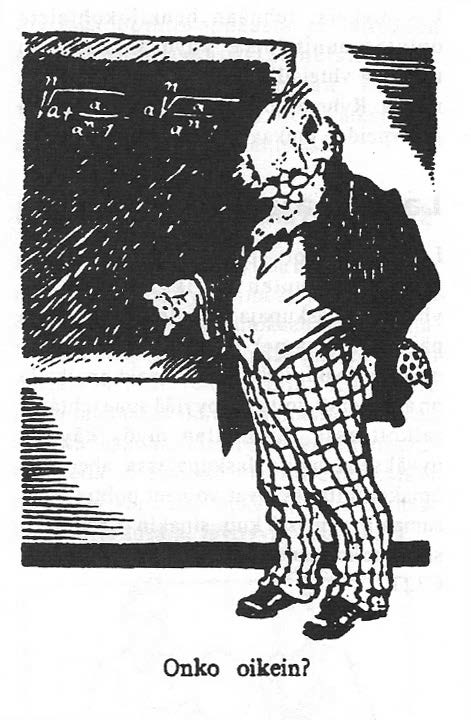
\includegraphics[width=\columnwidth]{onkooikein.png}
	\end{figure}
	
	FYMM~IIa kertaa aluksi tavallisia toisen
	asteen DY:itä, mutta pian päästään itse
	asiaan eli osittais\-differentiaali\-yhtälöihin
	ja niiden ratkaisuihin. Ennen kuin Legendren,
	Laguerren ja Hermiten polynomit
	ja ziljoonat Besselin funktiot on johdettu
	Frobeniuksen metodin avulla alkaa homma
	maistua puulta jossakin vaiheessa.
	
	Kannattaa silti roikkua mukana, sillä näitä erikois\-funktioita tarvitaan mm.\,elektro\-dynamiikassa,
	virtaus\-dynamiikassa sekä
	kvantti\-mekaniikassa.
	Loppuosassa luodaan ensin katsaus variaatio\-laskentaan,
	johon tutustutaan myös
	Klassisen mekaniikan kurssilla. Puolessa
	välissä kurssia Hilbertin avaruudet ja normien
	määrittelyt ilmestyvät aivan puun takaa,
	ja asiat jäävät pintaraapaisun tasolle ilman
	aiempia opintoja Exactumin puolella.
	
	\vspace{0.5cm}\noindent
	\textsc{Tommi Raita}\\
	\textsc{Aku Valtakoski}\\
	\textsc{Laura Aalto-Setälä}
	
	\subsubsection*{Kvanttimekaniikka~I (10~op)}
	Kvanttimekaniikka~I on useimpien
	mielestä teoreettisen fysiikan aine\-opintojen
	vaikein kurssi (taistelee ED:n kanssa
	ykkössijasta). Kvantti käydään yleensä
	kolmantena syksynä FYMMien
	jälkeen. Kurssi kelpaa myös fysiikan syventäviin
	opintoihin.
	\begin{figure}[t!]
		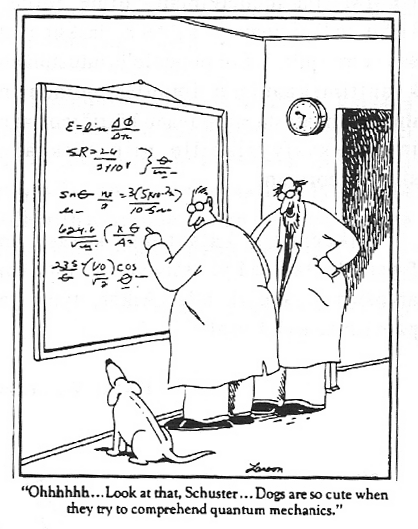
\includegraphics[width=\columnwidth]{dog_quantum.png}
	\end{figure}
	
	Kvantti on sisällöltään erittäin mielen\-kiintoinen,
	mutta laskuiltaan vaativa kurssi.
	Alussa kerrataan aalto\-mekaniikkaa, joka
	on monille tuttu aiemmilta kvantti\-fysiikan kursseilta, käsittelytapa
	vaan on täsmällisempi ja teoreettisempi.
	Seuraavaksi siirrytään Diracin formalismiin,
	joka lyhentää laskuja sen jälkeen kun
	sen oppii (jos oppii). Tämä osa on käsitteellisesti
	abstraktein. Muutaman sovelluksen
	jälkeen tutustutaan häiriö\-teoriaan ja sen
	sovelluksiin. Tässä vaiheessa on hyvä, jos
	on oppinut FYMMeillä brute
	force "-menetelmän laskujen läpi\-viemisen suhteen -- laskut
	ovat sen verran pitkiä.
	
	Jälkeenpäin katsottuna kurssi on fyysikolle
	tärkeää yleis\-sivistystä, jota voi arvostaa
	-- ja korkealle. Aikaa, työtä ja paperia se
	kyllä vaati.
	
	\vspace{0.5cm}\noindent
	\textsc{Harri Waltari}
	
	\subfile{sections/tahtitiede}
	\subfile{sections/meteorologia}
	\subfile{sections/geofysiikka}
\end{document}